\chapter{Experimentos y Detalles de Implementación}\label{chapter:implementation}

En este capítulo se presentan los experimentos realizados en la investigación para el desarrollo del sistema de segmentación, reconstrucción y medición de úlceras de pie diabético. Además, se presentan los resultados y argumentos sobre las decisiones tomadas en la propuesta final. En adición, se brindan detalles de la implementación y breves descripciones de las herramientas con que cuenta el software desarrollado.

Para el desarrollo de los experimentos se poseían dos computadoras: una de ellas con un CPU Intel\textregistered~Core\texttrademark~i5-8250U a 1.60GHz de 64-bit, con 8 Gb de RAM y con sistema operativo Ubuntu 20.04 LTS; la otra computadora con un CPU Intel\textregistered~Core\texttrademark~i7-4770HQ a 2.20GHz de 64-bit, con 16 Gb de RAM y sistema operativo MacOS 10.9.4. Además, para agilizar el procesamiento con las redes neuronales de la segmentación se contaba con la arquitectura de Google Colab con GPU NVIDIA K80. La cámara disponible era la Intel\textregistered~RealSense\texttrademark~D435i, la cual a distancias cortas provee mediciones de profundidad buenas para el desarrollo del proyecto; a diferencia de la cámara de profundidad de Microsoft \textit{Kinect v1} usada en~\cite{ching2022segm3d}, esta provee modelos 3D de calidad.

\section{Construcción del conjunto de datos}

Como seguimiento al trabajo~\cite{ching2022segm3d} se construyó un conjunto de datos que contiene secuencias de vídeo RGB-D de las úlceras de pie diabético. Las muestras se tomaron en el período de tiempo comprendido en los meses de abril a junio de 2022 en la consulta de angiología del INACV y el salón de curas de la sala ``Elpidio Sosa González'', en coordinación con los especialistas: Dr. José I. Fernández Montequín, Dr. Héctor T. Álvarez Duarte y Dr. Abraham Martínez.

En la captura de los datos era imprescindible obtener información relativa a la evolución de la UPD a lo largo del tiempo, por tal razón, se tomaron muestras de la misma úlcera con períodos de separación de mínimo una semana. Además, se obtuvieron datos relativos al paciente como nombre, edad, sexo, color de la piel, tipo de diabetes, tipo de úlcera, localización de la úlcera, así como la muestra de vídeo en RGB-D y el modelo 3D extraído con la cámara y el Intel\textregistered~RealSense\texttrademark~Viewer incluido en el SDK 2.0. Toda esta información se publica en el conjunto de datos a excepción del nombre del paciente, en su lugar se adjunta un código identificador compuesto por las iniciales del nombre, la edad y el sexo, por ejemplo: sea el paciente Susanny Vega Cintra de edad 25 años y sexo femenino, entonces su código de identificación es SVC-25-F.

El conjunto de datos está compuesto por 32 pacientes con edad promedio de 63 años; de estos pacientes, 23 de ellos son de sexo masculino y 9 de sexo femenino. Los colores de piel de los pacientes tenidos en cuenta tienen la siguiente distribución: 20 pacientes de piel blanca, 6 de piel negra, 5 de piel mestiza y 1 de piel amarilla. Los pacientes en su mayoría son diabéticos de tipo II, con una representación de 29 individuos, 2 diabéticos de tipo I, y 1 paciente que no era diabético. Se tomaron 65 muestras de úlceras de los 32 pacientes. Las úlceras estudiadas en su mayoría son úlceras de pie diabético de tipo neuro-infeccioso. La distribución del tipo de úlceras es: 20 úlceras neuro-infecciosas, 8 isquémicas, 3 flebolinfáticas y 1 lesión combinada. Las úlceras tienen mayor presencia en el pie izquierdo con un total de 22 y 10 en el pie derecho, donde las zonas con mayor afectación son los dedos, el dorsal del pie y la planta del mismo (Figura \ref{fig:loc}).

\begin{figure}[ht]
	\centering
	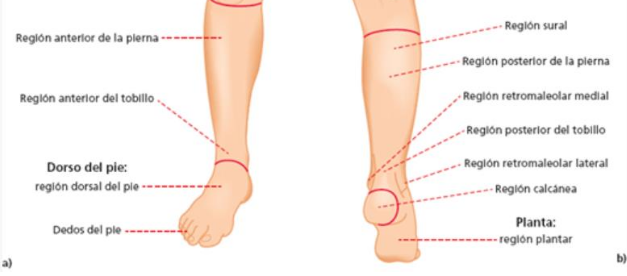
\includegraphics[width=10cm]{./Graphics/human.png}
	\caption{Las localizaciones anatómicas donde se presentan las lesiones}
	\label{fig:loc}
\end{figure}

Para la experimentación con la segmentación y la reconstrucción se tomaron 20 UPD del conjunto de datos anterior de 9 pacientes, y se extrajo un conjunto de imágenes RGB y de profundidad de las secuencias de vídeo. La extracción consistió en extraer uno de cada diez \textit{frames} del vídeo, por tal razón, se obtuvieron un total de 420 imágenes RGB y de profundidad. Todas las imágenes RGB no poseían la calidad necesaria para la experimentación, por tal razón, se hizo una eliminación manual utilizando como criterios de calidad lo siguiente:

\begin{itemize}
	\item Ausencia de ruido por movimiento o \textit{motion noise}.
	\item Iluminación adecuada en la zona de ulcerosa, en este caso, se utilizó como medición de la iluminación la perspectiva del ojo de quien realizó la eliminación. 
	\item Úlcera completamente visible. 
\end{itemize}

Las imágenes que incumplieran uno o varios de los criterios de calidad se descartaron. Luego de filtrar el conjunto con el criterio anterior se obtuvo un subconjunto de 253 imágenes. Para el proceso de segmentación era necesario obtener el \textit{ground truth} o segmentación verdadera de las imágenes. Para ello se elaboraron se forma manual un total de 135 \textit{ground truth} que fueron validadas por los especialistas. Sobre este conjunto de 135 imágenes con sus respectivos \textit{ground truth} validados se realizaron todos los procedimientos de experimentación.

\section{Experimentos e implementación de la segmentación de UPD}

Los experimentos desarrollados con el algoritmo de segmentación abarcan la evaluación de la capacidad del modelo de predecir los bordes de la úlcera en las imágenes obtenidas con las cámaras de profundidad. En caso, de reportarse un mal o ineficiente rendimiento del modelo con las nuevas imágenes se exploran técnicas de preprocesamiento, así como de asistencia al algoritmo para que se enfoque en la región de interés. Además, se exploran las razones de los fallos del algoritmo de segmentación. 

\subsection{Experimentación con el algoritmo de segmentación}

La experimentación con el algoritmo de segmentación incluye la predicción y el análisis de las métricas expuestas en la Sección \ref{sec:evalSeg}. 

El primer experimento que se desarrolló fue introducir las imágenes RGB como entrada al algoritmo de segmentación para observar la salida del mismo. Las máscaras resultantes aunque en la mayoría de los casos contenía de forma parcial o total la úlcera (obteniendo valores de Jaccard y Dice aceptables), además tenía grandes regiones de ruido que afectarían el resultado final de la reconstrucción y medición. Por tanto, se analizaron los factores de ruido en los que el algoritmo estaba fallando. 

Las redes neuronales fueron entrenadas en imágenes que solo contenían úlceras y no información del contexto, como pueden ser las camillas, los utensilios médicos, el piso de la consulta. En muchas ocasiones las texturas y colores de estos objetos son semejantes a los de las úlceras. En la Figura \ref{fig:confussion} se presenta una úlcera y el piso que está presente en esa imagen de la muestra, como se muestra los histogramas son bien parecidos con un coeficiente de correlación positiva de $0.6810$ aproximadamente. La mejora de contraste en las imágenes eliminó ruido de las mismas, pero no lo suficiente.

\begin{figure}
	\centering
	\begin{subfigure}
		\centering
		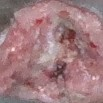
\includegraphics[width=.3\linewidth]{./Graphics/expdfu.jpg}
	\end{subfigure}
	\begin{subfigure}
		\centering
		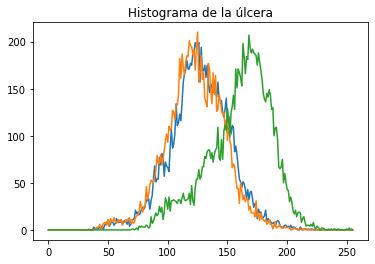
\includegraphics[width=.5\linewidth]{./Graphics/histDFU.png}
	\end{subfigure}
	\begin{subfigure}
		\centering
		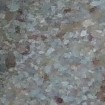
\includegraphics[width=.3\linewidth]{./Graphics/floor.jpg}
	\end{subfigure}
	\begin{subfigure}
		\centering
		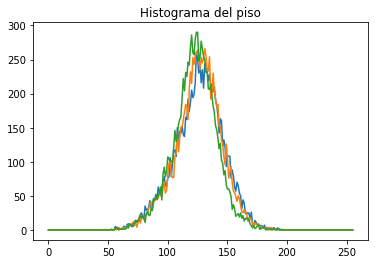
\includegraphics[width=.5\linewidth]{./Graphics/histFloor.png}
	\end{subfigure}
	\caption{Zonas confusas: (arriba) la úlcera y su histograma, (abajo) piso y su histograma}
	\label{fig:confussion}
\end{figure}

Otra de las regiones de confusión para el algoritmo es el pañuelo verde que se coloca en las consultas para realizar las curas y tomar las muestras (Figura \ref{fig:tissueMask} (izquierda)). Al ocasionar problemas el pañuelo, se decidió eliminarlo de las imágenes utilizando segmentación de umbral en los colores del pañuelo. 

\begin{figure}
	\centering
	\begin{subfigure}
		\centering
		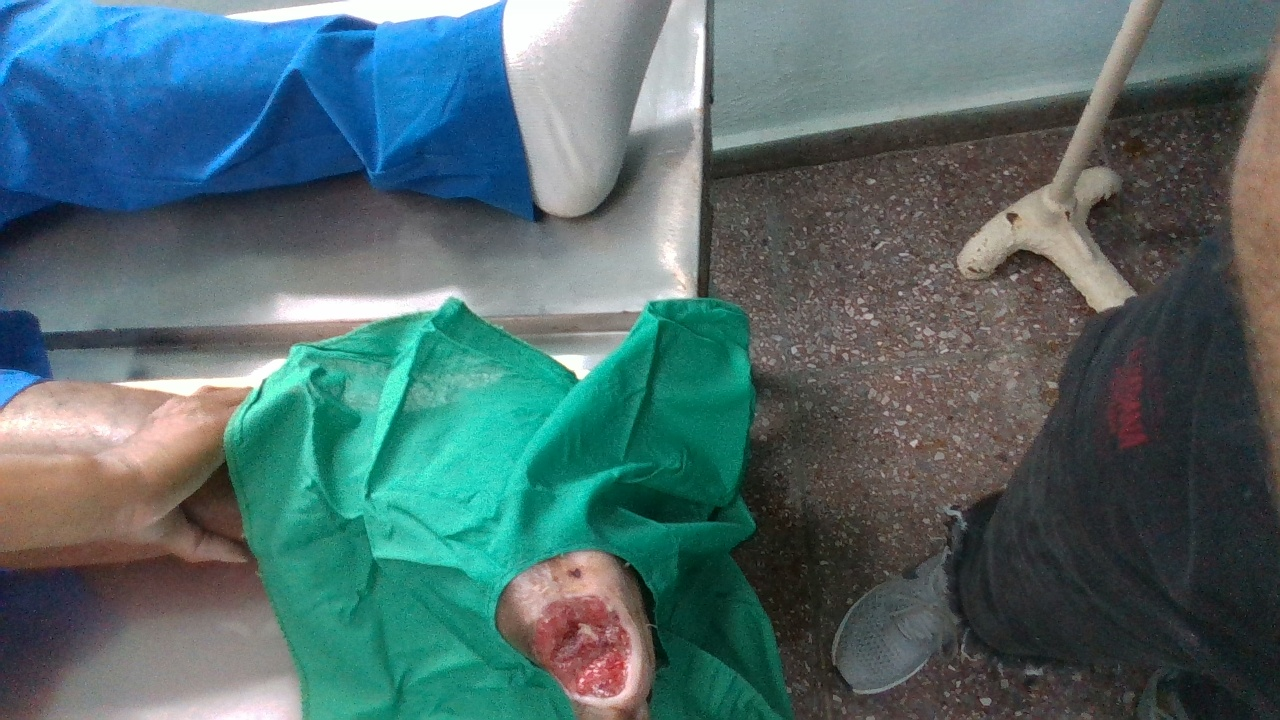
\includegraphics[width=.4\linewidth]{./Graphics/tissue.jpg}
	\end{subfigure}
	\begin{subfigure}
		\centering
		
\includegraphics[width=.4\linewidth]{./Graphics/tissueMask.jpg}
	\end{subfigure}
	\caption{Imagen donde se observa el pañuelo verde (Izquierda) y la máscara de segmentación (Derecha)}
	\label{fig:tissueMask}
\end{figure}

Para evitar estos problemas se decidió utilizar un enfoque asistido de segmentación en el cual el especialista define la región de interés para el algoritmo, o sea, recorta la imagen de forma que solo quede la úlcera en su centro. Además, se utiliza la mejora de contraste, el filtro de \textit{sharpening} para acentuar los bordes de las imágenes y la eliminación del pañuelo. Se obtienen las métricas que se muestran en la tabla siguiente.

\begin{table}[ht]
	\centering
	\begin{tabular}{lll}
		\hhline{===}
		& INACV\\
		\hhline{===}
		Jaccard medio & 84.55 \% \\ \hline
		F1-Score medio & 88.29 \% \\ \hline
		Precisión media& 88.04 \% \\
		\hline
		Recobrado medio & 91.54 \\
		\hline
	\end{tabular}
	\caption{Métricas de evaluación de la segmentación en el conjunto de datos obtenidos en el INACV}
	\label{tab:metricSegm}
\end{table}

Como alternativa al enfoque asistido de segmentación se experimentó la alternativa propuesta en~\cite{filko2018wound}. Este método propone construir subimágenes de tamaño 16 $\times$ 16 de cada \textit{frame} y entrenar el algoritmo kNN con la distancia de Bhattacharyya y $k = 7$ para predecir la localización de la úlcera. Pero debido a los problemas referidos a las zonas de confusión no dió resultados admisibles. Otro de los enfoques con los que se experimentó es utilizar las imágenes de profundidad para eliminar el ruido en las imágenes RGB. Este enfoque se probó pero no arrojó de igual manera resultados concluyentes. Por estas razones se decidió por la alternativa asistida y el algoritmo de seguimiento de objetos en secuencias de vídeo.

\subsection{Optimización del uso de la memoria RAM}

Todo el proceso de experimentación de la segmentación se desarrolló en \textit{Google Colab} haciendo uso de las Unidades Gráficas de Procesamiento (GPU). Al ejecutar la implementación utilizando los ordenadores disponibles, se enfrentó un problema de sobrecarga de la memoria RAM de los dispositivos, 8 y 16 gigabytes respectivamente.

La implementación que ocasionaba la sobrecarga almacenaba en memoria las 10 redes neuronales con los pesos correspondientes a la segmentación. Esto traía consigo que el programa en los dispositivos que se tienen a disposición se cerrara debido al llenado de la RAM. Se cambió dicha implementación a cambio de sacrificar la velocidad de cómputo.

El cambio que se introdujo es la carga de las redes neuronales y sus pesos, uno a la vez en demanda, o sea, cuando se necesita la red $i$-ésima para realizar la predicción se carga a la memoria. De esta forma, se reduce el consumo de la RAM garantizando que exista solo una red en un momento dado y es la que se va a utilizar.

\section{Resultados y detalles de la implementación de la reconstrucción 3D}\label{sec:resRec3d}

Para realizar la reconstrucción, el algoritmo propuesto utiliza hiperparámetros que influyen al momento de generar la malla. Para cada paso de la reconstrucción se analizaron los valores con los que se optimizaba el proceso en cuanto a calidad de la malla y tiempo de ejecución.

\subsection{Creación de fragmentos}

En el primer paso de la reconstrucción se crean los fragmentos, para esto es necesario indicar cada cuantos \textit{frames} se va a generar un fragmento, por lo que se introduce el parámetro \verb|n_frames_per_fragment|. Las muestras tomadas en el INACV varían entre 40 y 80 \textit{frames}. Se observa además, que el procedimiento obtiene mejores resultados con 3-4 fragmentos, de aquí que se estime la creación de un fragmento cada 20 $frames$.

Se introduce también el parámetro \verb|max_depth|, los valores de profundidad mayores que \verb|max_depth| serán truncados a cero. Teniendo en cuenta que las muestras se obtienen a una distancia de $20\text{cm}$ a $30\text{cm}$, se puede estimar este valor como $85\text{cm}$.

La odometría RGBD calcula el movimiento de la cámara entre dos imágenes RGBD consecutivas, en \textit{Open3D} se encuentran disponibles dos métodos:~\cite{steinbrucker2011real} y~\cite{park2017colored}, siendo este último el que mejores resultados obtiene en la mayoría de los conjuntos de datos. En el dominio de la imagen de profundidad, si dos píxeles alineados tienen una diferencia de profundidad menor que un valor especificado, se considera una correspondencia. Un valor más grande induce una búsqueda más agresiva, pero es propenso a resultados inestables. De aquí se deduce otro parámetro útil \verb|max_depth_diff|, con un valor de $3\text{mm}$.

Para finalmente generar el volúmen TSDF del fragmento, se necesita precisión, por lo que se precisan \textit{voxels} de 1mm aproximadamente, para esto se define el tamaño del TSDF cúbico a 0.5m, con lo que se obtiene $\frac{0.5\text{mm}}{512}$ aproximadamente 1mm.

\subsection{Registro y refinamiento de fragmentos}

Para preprocesar los fragmentos como nubes de puntos se reduce la muestra a un nuevo tamaño de voxel, se llama a este parámetro como \verb|voxel_size|. Aquí nuevamente se busca precisión, por lo que se intenta no reducir la muestra y asignar el valor real de 1mm, y este será el valor usado para todos los procesos posteriores.

En \textit{Open3D} se tienen dos procedimientos disponibles para el registro ICP: \textit{punto a punto}~\cite{besl1992method}  y \textit{punto a plano}~\cite{chen1992object}, en~\cite{rusinkiewicz2001efficient} se muestra que el algoritmo \textit{punto a plano} para ICP converge con mayor rapidez que \textit{punto a punto}. Recientemente, en~\cite{park2017colored} se introduce una variante para ICP, que usa tanto las características geométricas como el color para el registro, la información de color cierra la alineación a lo largo del plano tangente. Por lo tanto, este algoritmo es más preciso y más robusto que los algoritmos de registro de nubes de puntos anteriores, mientras que la velocidad de ejecución es comparable a la del registro ICP. Luego el parámetro \verb|icp_method| apuntará al último algoritmo descrito.

Tanto el registro ICP como la variante vista anteriormente se conocen como métodos de registro local porque se basan en una alineación aproximada como inicialización. Existe otra clase de métodos de registro, conocida como registro global. Esta familia de algoritmos no requiere una alineación para la inicialización. Por lo general, producen resultados de alineación menos estrictos y se utilizan como inicialización de los métodos locales. La elección de este método se debate entre RANSAC y Registro Global Rapido (FGR) introducido en~\cite{zhou2016fast}. La solución de registro global basada en RANSAC puede llevar mucho tiempo debido a las innumerables propuestas y evaluaciones de modelos. En~\cite{zhou2016fast} se introdujo un enfoque más rápido que optimiza rápidamente los pesos de proceso de línea de pocas correspondencias. Como no hay una propuesta de modelo ni una evaluación para cada iteración, el enfoque propuesto en~\cite{zhou2016fast} puede ahorrar mucho tiempo computacional. Con la configuración apropiada, la exactitud de FGR es incluso comparable a ICP, se pueden observar mas resultados en~\cite{zhou2016fast}.

\section{Resultados de los experimentos relativos a la medición de las UPD}

En la etapa de medición de las úlceras de pie diabético era necesario evaluar la precisión de las mediciones a través de los modelos tridimensionales obtenidos con las cámaras de profundidad y el proceso de reconstrucción. 

\subsection{Generación de tapas para las UPD}

La generación de las tapas de las úlceras de pie diabético constituyen un paso importante en el algoritmo para la estimación del volumen de la misma. La implementación del algoritmo de generación consiste en la detección de los puntos del borde de la malla poligonal de la úlcera que se asume coinciden con los bordes de la úlcera. Estos puntos se detectan anulando la componente $z$ de los puntos de la malla, luego se calcula la envoltura convexa de la imagen plana y los bordes son aquellos puntos que se localicen sobre la envoltura convexa. Posteriormente, se aplica un \textit{spline} cúbico para interpolar la superficie de la tapa.

Se definen dos tipos de úlceras teniendo en cuenta la forma de la cavidad, con el fin de explicar los resultados de la generación de las tapas, para ello se toma como referencia un plano imaginario ($T_P$) que se traza interpolando los puntos del borde de la UPD:

\begin{itemize}
	\item \textit{Cóncavas:} aquellas úlceras en las cuales la superficie de su tapa se puede aproximar por un plano, debido a que la mayor parte de la úlcera está por debajo de $T_P$.(Figura \ref{fig:planar} (izquierda)).
	\item \textit{Convexas:} aquellas úlceras en las cuales la superficie de su tapa no se puede aproximar por un plano, debido a que la mayor parte de la UPD está por encima de $T_P$. (Figura \ref{fig:planar} (derecha)).
\end{itemize}

\begin{figure}[ht]
	\centering
	\begin{subfigure}
		\centering
		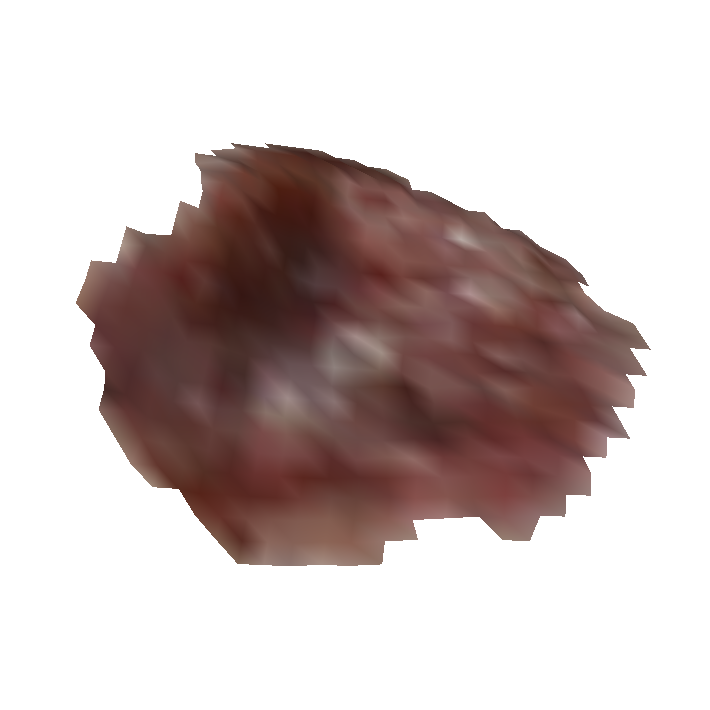
\includegraphics[width=.25\linewidth]{./Graphics/planar.png}
	\end{subfigure}
	\begin{subfigure}
		\centering
		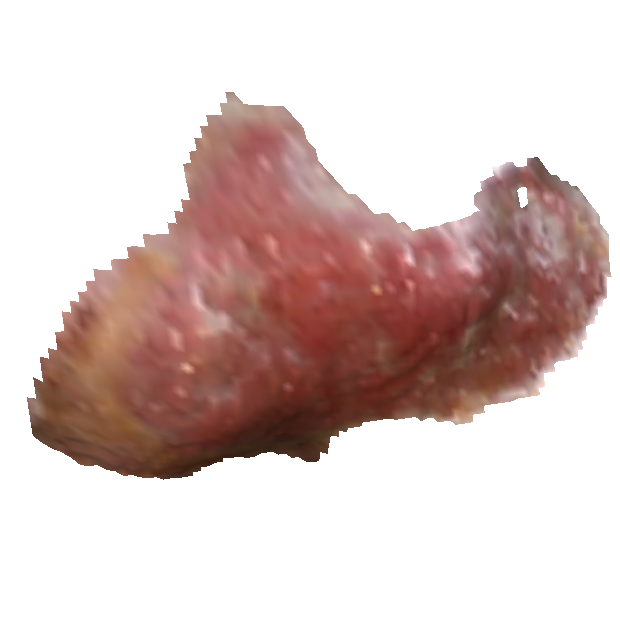
\includegraphics[width=.25\linewidth]{./Graphics/noPlanar.png}
	\end{subfigure}
	\caption{Tipos de UPD según la forma de su cavidad: (izquierda) UPD cóncava, (derecha) UPD convexa.}
	\label{fig:planar}
\end{figure}

Se tomaron 10 úlceras del conjunto de datos, de pacientes distintos para realizar experimentos sobre la generación de la tapa. Este experimento se evalúa con información brindada por los especialistas sobre la superficie de cicatrización y granulación de las UPD, debido a que no se cuenta con las superficies verdaderas de las tapas.

Las tapas obtenidas para úlceras cóncavas estiman bastante bien la superificie (Figura \ref{fig:planartops}), pues cubren toda la úlcera y se trazan cercanas al nivel que alcanzaría la cicatrización y granulación de la lesión. Sin embargo, con las úlceras convexas no se obtienen resultados satisfactorios (Figura \ref{fig:noplanartops}). 

\begin{figure}[ht]
	\centering
	\begin{subfigure}
		\centering
		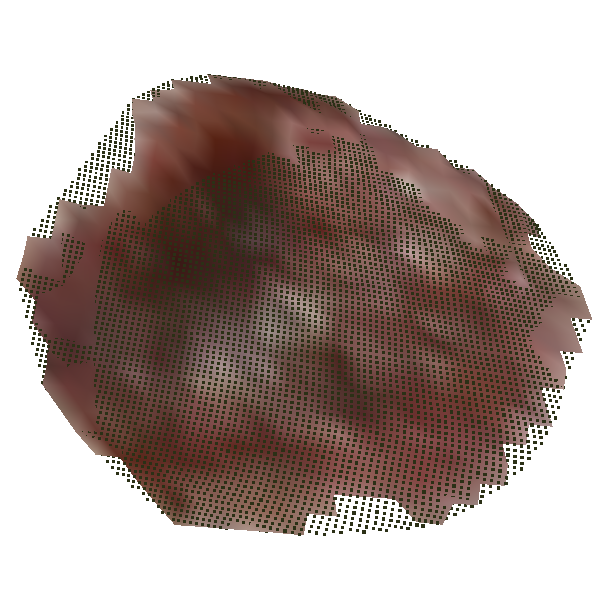
\includegraphics[width=.2\linewidth]{./Graphics/planar01.png}
	\end{subfigure}
	\begin{subfigure}
		\centering
		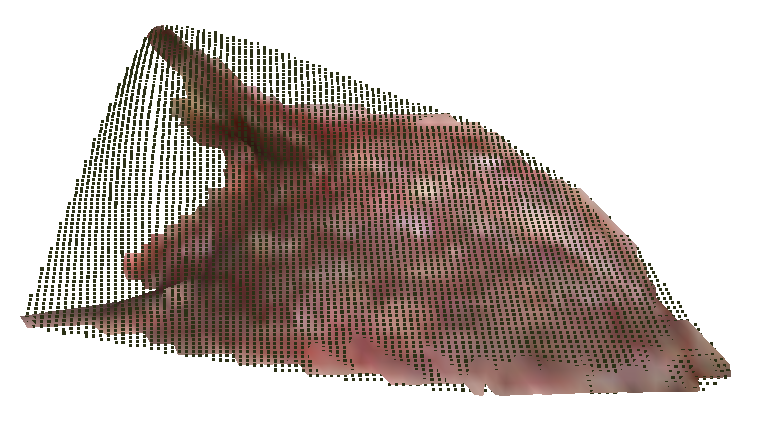
\includegraphics[width=.2\linewidth]{./Graphics/planar03.png}
	\end{subfigure}
	\begin{subfigure}
		\centering
		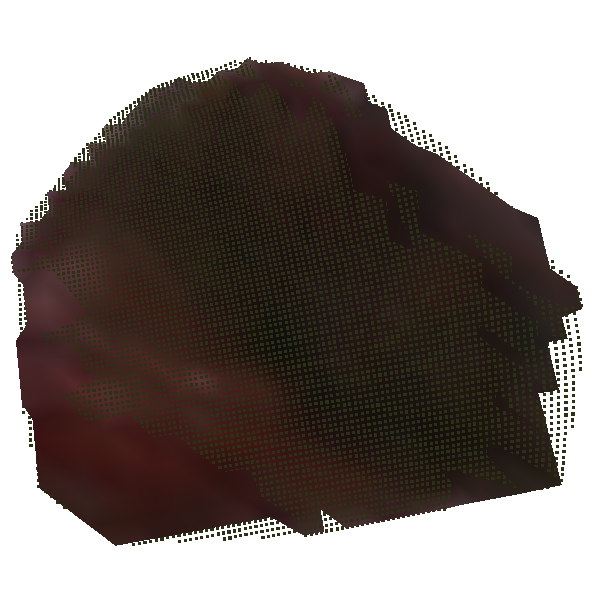
\includegraphics[width=.2\linewidth]{./Graphics/planar02.png}
	\end{subfigure}
	\begin{subfigure}
		\centering
		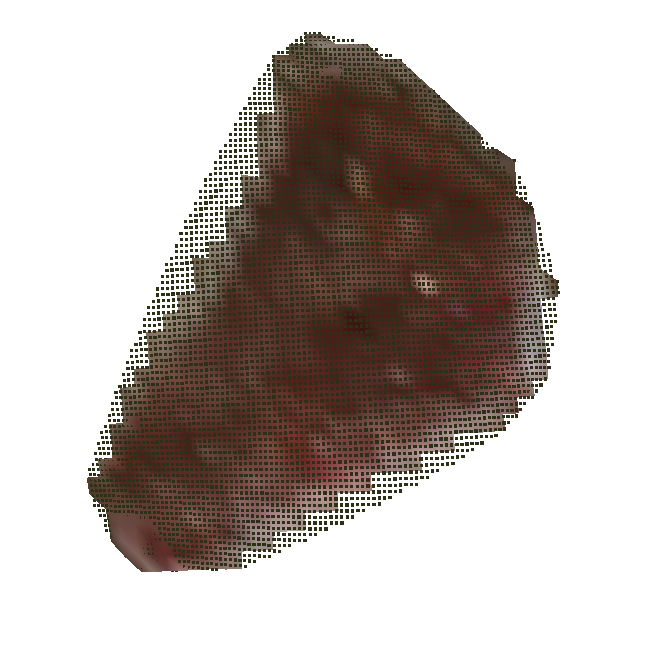
\includegraphics[width=.2\linewidth]{./Graphics/planar04.png}
	\end{subfigure}
	\caption{Estimación de la tapa de úlceras cóncavas.}
	\label{fig:planartops}
\end{figure} 

\begin{figure}[ht]
	\centering
	\begin{subfigure}
		\centering
		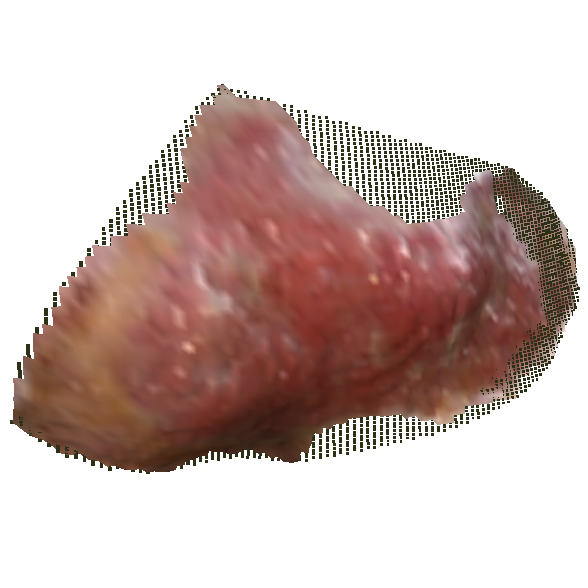
\includegraphics[width=.2\linewidth]{./Graphics/noplanar02.png}
	\end{subfigure}
	\begin{subfigure}
		\centering
		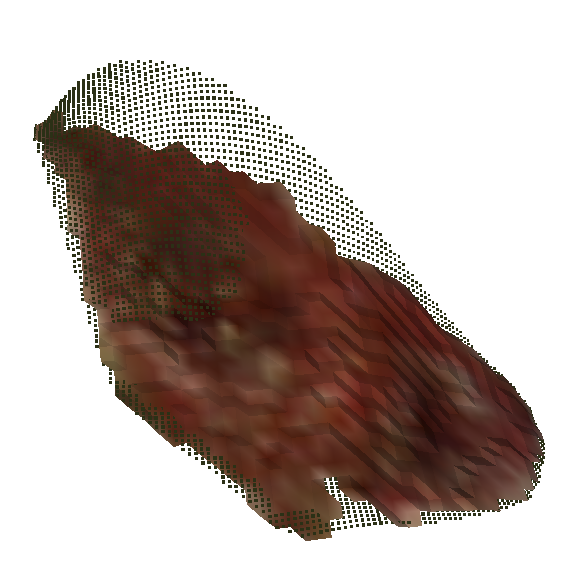
\includegraphics[width=.18\linewidth]{./Graphics/noplanar01.png}
	\end{subfigure}
	\begin{subfigure}
		\centering
		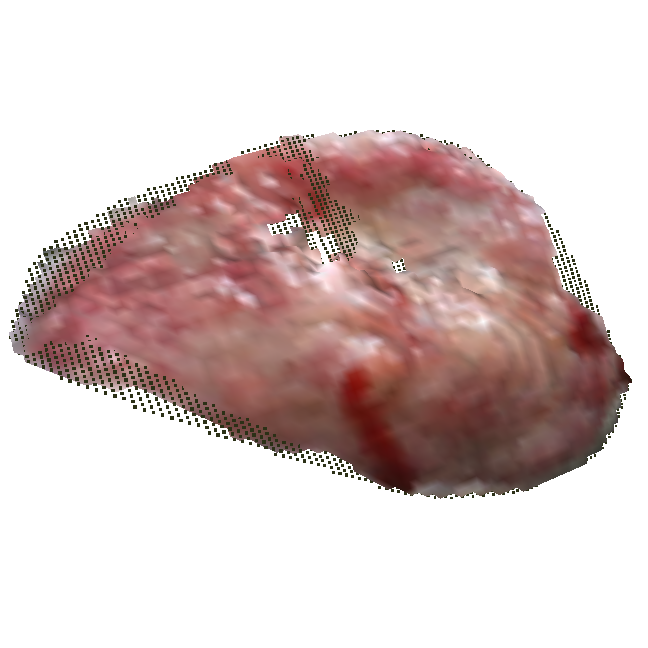
\includegraphics[width=.2\linewidth]{./Graphics/noplanar03.png}
	\end{subfigure}
	\begin{subfigure}
		\centering
		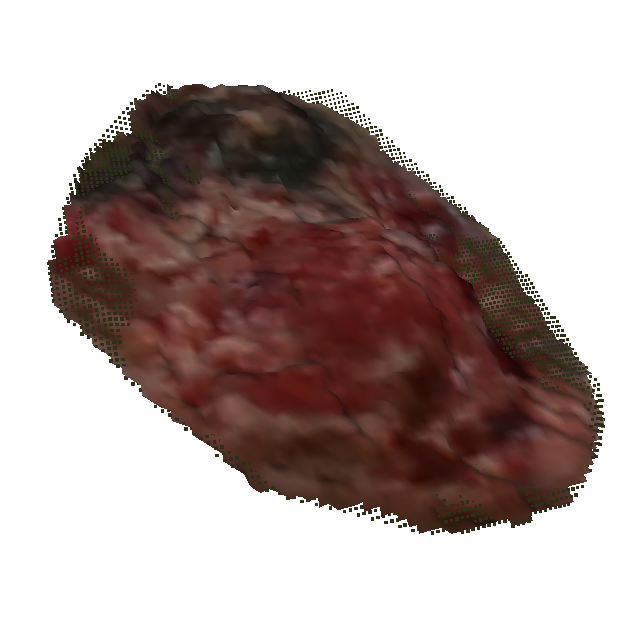
\includegraphics[width=.18\linewidth]{./Graphics/noplanar05.png}
	\end{subfigure}
	\caption{Estimación de la tapa de úlceras convexas. }
	\label{fig:noplanartops}
\end{figure} 

Esto ocurre debido a que la interpolación se ejecuta solo con los datos del borde de la úlcera lo que no aporta información de relativa a la ubicación de la cavidad de la lesión. Por esto se exploró otra alternativa, calcular la envoltura convexa de la malla de la úlcera e interpolar sobre los puntos que se encuentran sobre la envoltura convexa. Este enfoque aporta mejores resultados en la generación de tapas, en particular en las lesiones convexas, pero aumenta el error en la medición de úlcera cóncavas y en el experimento de precisión que se describe en la Sección \ref{sec:expPrec}. Por esta razón, se decidió adoptar con el enfoque anterior priorizando las úlceras cóncavas.

\subsection{Evaluación de la precisión de las mediciones}\label{sec:expPrec}

La medición de las úlceras de pie diabético a través de la reconstrucción 3D necesita ser precisa, con el fin de validar el sistema y aportar información de valor a los especialistas que les ayude a realizar un seguimiento de la evolución del paciente. Por tanto, se realizó un experimento para evaluar la precisión del sistema en medir perímetro, área y volumen. 

Para la experimentación es necesario poseer datos acerca del valor numérico real de los estimadores geométricos de una o varias úlceras. Debido a la inexistencia de los datos o un método para la medición, se utilizó como objeto una pieza de poliespuma con una cavidad con forma de cilindro circular recto de diámetro de $d = 4$cm y altura $h = 1.1$cm (Figura \ref{fig:recObj}). Los valores numéricos de las mediciones reales del objeto son:

\begin{itemize}
	\item Perímetro ($P$): la cavidad tiene forma de circunferencia, por tanto, se calcula $P = P_{circ} = 2\pi r$ donde $r$ es el radio de la circunferencia. Por tal razón, el perímetro es $$P = 2\pi * 20\text{mm} = 40\pi\text{mm}$$
	\item Área ($A$): la cavidad tiene forma de cilindro circular recto, por tanto, su área se calcula como el área total de la superficie menos el área de la base del cilindro. La ecuación quedaría:
	$$A = A_{cil_{L}} + A_{cil_{B}} =  2\pi rh + \pi r^2 = 440 \pi \text{mm}^2 + 400\pi \text{mm}^2 = 840 \pi\text{mm}^2$$ 
	\item Volumen ($V$): la cavidad es un cilindro circular recto, por tanto, se calcula $$V = V_{cil} = \pi r^2 h = 400\pi 
	* 11 \text{mm}^3 = 4400\pi \text{mm}^3$$
\end{itemize}

Estos valores se obtuvieron midiendo de forma directa el diámetro y la altura del objeto, luego, aplicando las fórmulas geométricas correspondientes. 

\begin{figure}[ht]
	\centering
	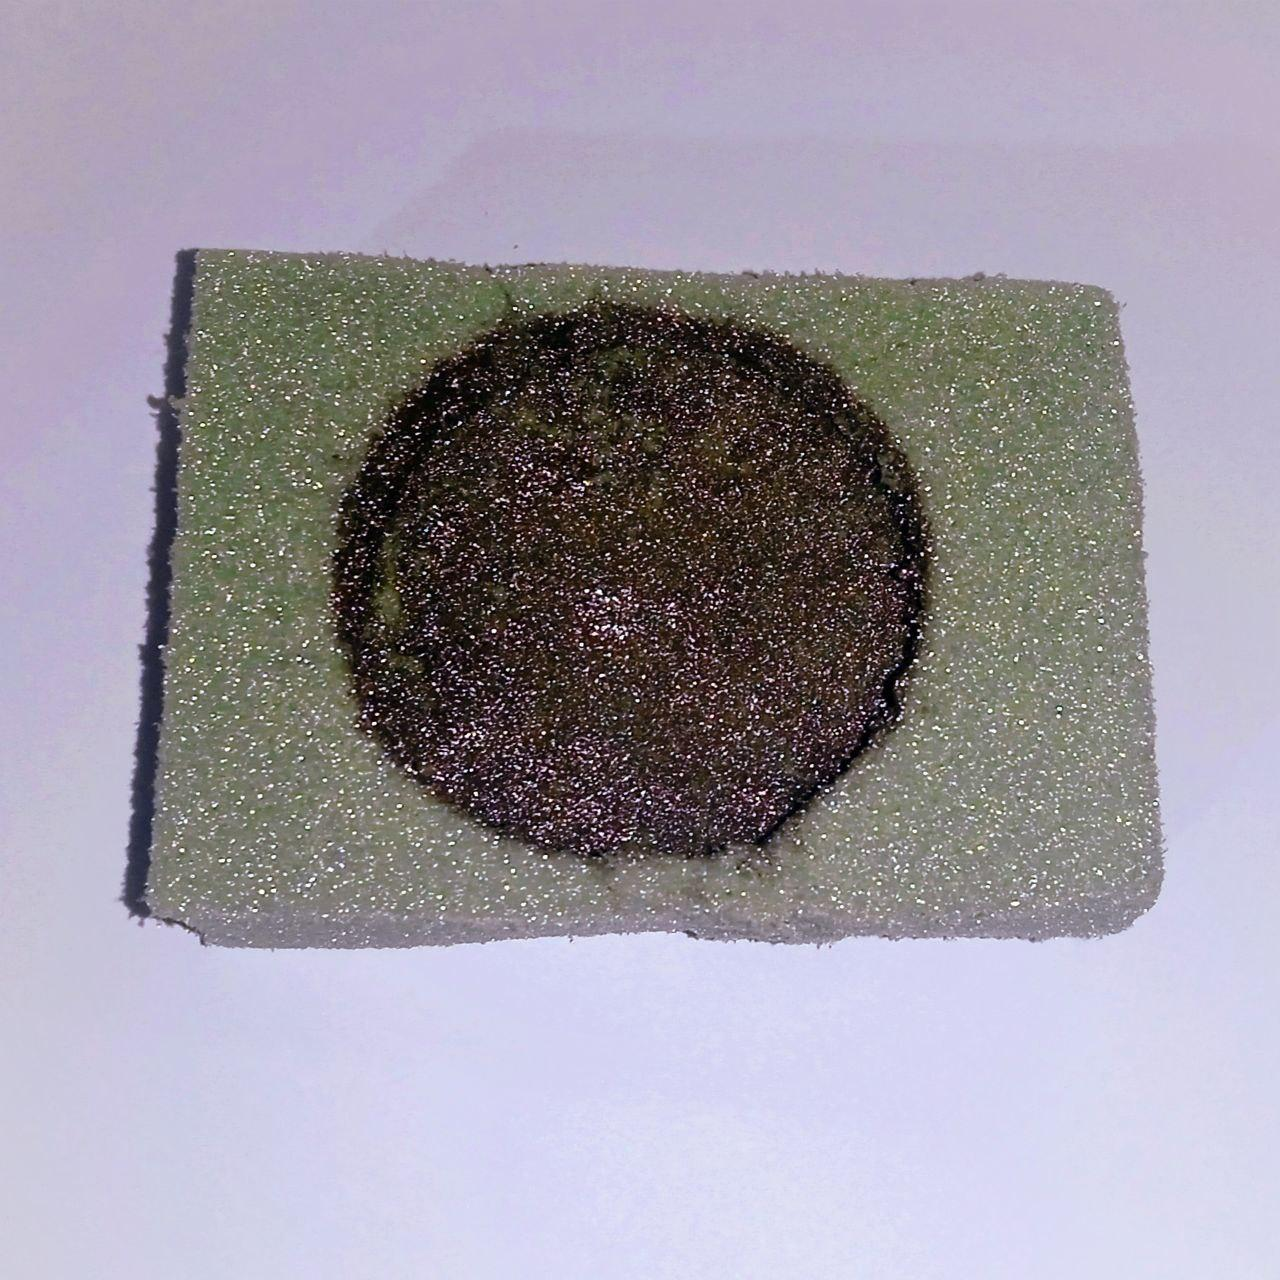
\includegraphics[width=4cm]{./Graphics/reconstruction-object.jpg}
	\caption{Objeto de prueba del experimento}
	\label{fig:recObj}
\end{figure}

El experimento consiste en realizar la reconstrucción 3D del objeto para obtener su modelo, medir y luego, comparar con los valores numéricos reales para calcular el error cometido. Es necesario conocer también la estabilidad de la medición, esto es que al realizar el proceso sobre el mismo objeto siempre se cometa el mismo error de aproximación. Por tal razón, se añade al experimento una etapa en la que se repite el proceso descrito anteriormente una cantidad $n$ de veces y luego se halla la media y desviación estándar del error cometido en cada instancia del experimento.

Se tomaron $n = 20$ secuencias de vídeo RGB-D haciendo distintos recorridos, comenzando la secuencia en diferentes puntos de vista y a diferentes distancias del objetivo siempre manteniendo el rango recomendado. Se realizaron las reconstrucciones correspondientes de la escena, obteniéndose los modelos 3D. De forma manual, se eliminaron de los modelos aquellos vértices que no corresponden a la zona de la cavidad. Posteriormente, se procedió a medir perímetro, área y volumen. 

Los resultados del experimento se describen a continuación. Se tomó como valor de la constante matemática $\pi$ la aproximación que brinda la implementación de \textit{Numpy} en la versión 1.23.3. Se analizan los resultados en cada uno de los estimadores.

\subsubsection{Perímetro}

En la aproximación del perímetro se esperaba un resultado de $40\pi\text{mm}$ que es $125.66370614359172\text{mm}$. Se obtuvo un error absoluto ($\epsilon_A$) máximo de $16.3324\text{mm}$ aproximadamente, que representa un error relativo ($\epsilon_R$) de $12.9969\%$ aproximadamente; por otro lado, el error absoluto mínimo que se consiguió es de aproximadamente $1.5876\text{mm}$ lo que representa un error relativo de $1.2634\%$. El error absoluto medio es aproximadamente de $10.5401\text{mm}$ lo que representa un error relativo de $8.3876\%$, la mediana del error absoluto es aproximadamente de $11.0085\text{mm}$ que representa un error relativo de un $8.7603\%$. La Figura \ref{fig:histP} muestra el histograma de frecuencias de las mediciones del perímetro y el error absoluto.

\begin{figure}[ht]
	\centering
	\begin{subfigure}
		\centering
		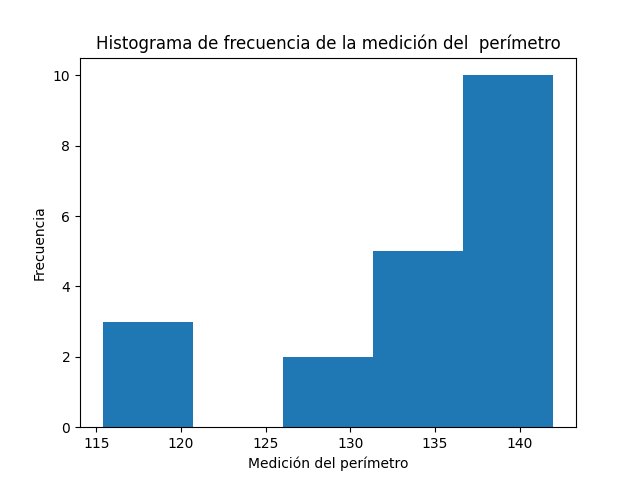
\includegraphics[width=.49\linewidth]{./Graphics/histP.png}
	\end{subfigure}
	\begin{subfigure}
		\centering
		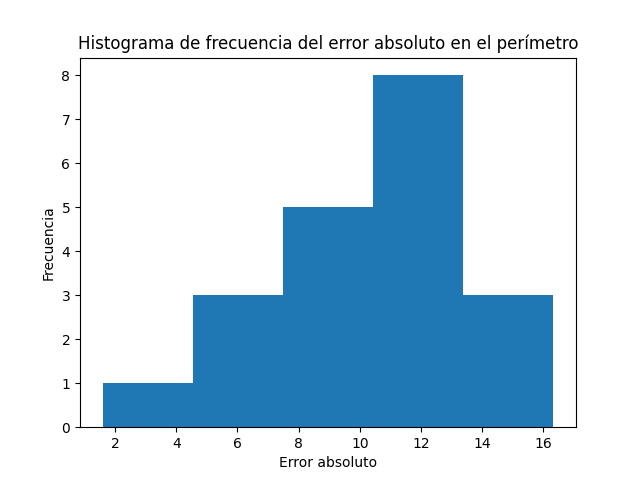
\includegraphics[width=.49\linewidth]{./Graphics/histPEA.png}
	\end{subfigure}
	\caption{Histogramas de frecuencia correspondientes al análisis de la medición del perímetro. (Izquierda) histograma de la medición y (Derecha) histograma del error absoluto.}
	\label{fig:histP}
\end{figure}

Como se observa en la Figura \ref{fig:histP} (Izquierda) la tendencia en la muestra es estimar el perímetro por encima del valor real. El intervalo de confianza de la media del error relativo es $[7.0835\%, 9.6916\%]$ con $\alpha =0.95$. Por esta razón se concluye que el error relativo que se comete al aproximar el perímetro es de $8.3876\% \pm 1.3040\%$. 

Luego, al analizar la dispersión de las mediciones se encuentra que la media de las aproximaciones es $133.5361\text{mm}$ que contiene $\epsilon_R=6.2646\%$ y la desviación típica con respecto a esta media es $7.7953\text{mm}$. Por tal razón, en un conjunto de mediciones de una misma úlcera se puede concluir que se van a obtener valores con desviación estándar $7.7953\text{mm}$ de la media que ya tiene un error de aproximación descrito anteriormente.

\subsubsection{Área}


En la aproximación del área del objeto se esperaba un resultado de $840\pi\text{mm}^2$ que es $2638.9378290154264\text{mm}^2$. Se obtuvo un error absoluto ($\epsilon_A$) máximo de aproximadamente $1300.6449\text{mm}^2$, que representa un error relativo ($\epsilon_R$) de $49.2866\%$ aproximadamente; por otro lado, el error absoluto mínimo que se consiguió es de aproximadamente $8.0087\text{mm}^2$ lo que representa un error relativo de $0.3034\%$. El error absoluto medio es aproximadamente de $470.9007\text{mm}^2$ lo que representa un error relativo de $17.8443\%$, la mediana del error absoluto es aproximadamente de $428.6708\text{mm}^2$ que representa un error relativo de un $16.2440\%$. La Figura \ref{fig:histA} muestra el histograma de frecuencias de las mediciones del área y el error absoluto.

\begin{figure}[ht]
	\centering
	\begin{subfigure}
		\centering
		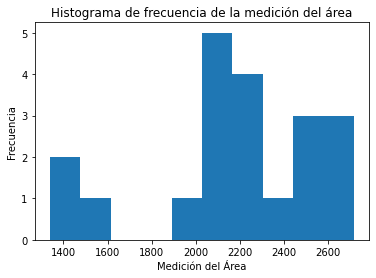
\includegraphics[width=.49\linewidth]{./Graphics/histA.png}
	\end{subfigure}
	\begin{subfigure}
		\centering
		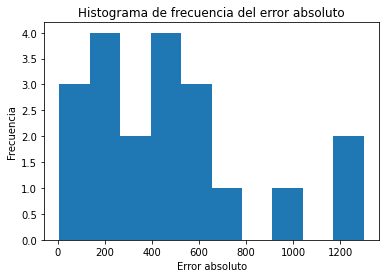
\includegraphics[width=.49\linewidth]{./Graphics/histAEA.png}
	\end{subfigure}
	\caption{Histogramas de frecuencia correspondientes al análisis de la medición del área. (Izquierda) histograma de la medición y (Derecha) histograma del error absoluto.}
	\label{fig:histA}
\end{figure}

Como se observa en la Figura \ref{fig:histA} (Izquierda) la tendencia en la muestra es estimar el área por debajo del valor real. El intervalo de confianza de la media del error relativo es $[11.3237\%, 24.3648\%]$ con $\alpha =0.95$. Por esta razón se concluye que el error relativo que se comete al aproximar el área es de $17.8443\% \pm 6.5205\%$. 

Luego, al analizar la dispersión de las mediciones se encuentra que la media de las aproximaciones es $2181.3191\text{mm}^2$ que contiene $\epsilon_R=17.3410\%$ y la desviación típica con respecto a esta media es $375.1690\text{mm}^2$. Por tal razón, en un conjunto de mediciones de una misma úlcera se puede concluir que se van a obtener valores con desviación estándar $375.1690\text{mm}^2$ de la media que ya tiene un error de aproximación descrito anteriormente.

\subsubsection{Volumen}

En la aproximación del volumen se esperaba un resultado de $4400\pi\text{mm}^3$ que es $13823.00767579509\text{mm}^3$. Se obtuvo un error absoluto ($\epsilon_A$) máximo de aproximadamente $7421.2339\text{mm}^3$, que representa un error relativo ($\epsilon_R$) de $53.6875\%$ aproximadamente; por otro lado, el error absoluto mínimo que se consiguió es de aproximadamente $314.7221\text{mm}^3$ lo que representa un error relativo de $2.2767\%$. El error absoluto medio es aproximadamente de $3289.5647\text{mm}^3$ lo que representa un error relativo de $23.7977\%$, la mediana del error absoluto es aproximadamente de $2672.1483\text{mm}^3$ que representa un error relativo de un $19.3311\%$. La Figura \ref{fig:histV} muestra el histograma de frecuencias de las mediciones del volumen y el error absoluto.

\begin{figure}[ht]
	\centering
	\begin{subfigure}
		\centering
		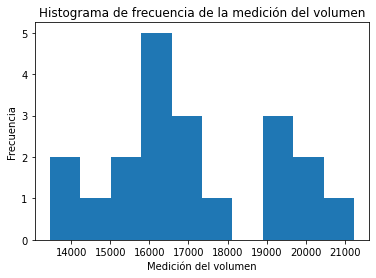
\includegraphics[width=.49\linewidth]{./Graphics/histV.png}
	\end{subfigure}
	\begin{subfigure}
		\centering
		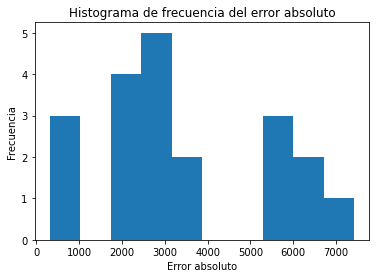
\includegraphics[width=.49\linewidth]{./Graphics/histVEA.png}
	\end{subfigure}
	\caption{Histogramas de frecuencia correspondientes al análisis de la medición del volumen. (Izquierda) histograma de la medición y (Derecha) histograma del error absoluto.}
	\label{fig:histV}
\end{figure}

Como se observa en la Figura \ref{fig:histA} (Izquierda) la tendencia en la muestra es estimar el volumen por encima del valor real. El intervalo de confianza de la media del error relativo es $[16.7570\%, 30.8384\%]$ con $\alpha =0.95$. Por esta razón se concluye que el error relativo que se comete al aproximar el área es de $23.7977\% \pm 7.0407\%$. 

Luego, al analizar la dispersión de las mediciones se encuentra que la media de las aproximaciones es $17043.4887\text{mm}^3$ que contiene $\epsilon_R=23.2979\%$ y la desviación típica con respecto a esta media es $2134.9136\text{mm}^3$. Por tal razón, en un conjunto de mediciones de una misma úlcera se puede concluir que se van a obtener valores con desviación estándar $2134.9136\text{mm}^3$ de la media que ya tiene un error de aproximación descrito anteriormente.


\begin{table}[ht]
	\centering
	\begin{tabular}{lll}
		\hhline{===}
		& Error absoluto medio & Error relativo medio\\
		\hhline{===}
		Perímetro & $10.5401\text{mm} \pm 1.4250\text{mm}$ & $8.3876\% \pm 1.3040\%$ \\ \hline
		Área & $470.9007\text{mm}^2 \pm 172.0728\text{mm}^2$ & $17.8443\% \pm 6.5205\%$\\ \hline
		Volumen & $3289.5647\text{mm}^3 \pm 973.2375\text{mm}^3$ & $23.7977\% \pm 7.0407\%$\\
		\hline
	\end{tabular}
	\caption{Resumen del error cometido en las mediciones}
	\label{tab:err}
\end{table}
